\chapter{The Data Manager}
The Data Manager\index{Data Manager tab}\index{Graphical User Interface (GUI)!Data Manager tab}
has two primary purposes, each reflected in the sub-tabs.  One tab, the 
Opus Data tab, is for browsing, viewing, and exporting data from the Opus data cache.  
The other tab, the Tools tab,
is a place for storing and executing 
various tools provided by the Opus community or tools you have written.

\section{Opus Data Tab}\index{Opus Data tab}\index{Graphical User Interface (GUI)!Opus Data tab}

The Opus Data tab is a file browser that defaults to the folder in which
your project creates data.  This folder name is composed from the default 
location for the Opus files, followed by \file{data}, followed by the project
name.  The project name for the \file{eugene_gridcell_default.xml} project is
``eugene\_gridcell.'' (This is given in the ``project\_name'' element in the xml.)
Thus, if you installed to
\file{c:/opus}, and you are opening the Eugene sample project at
\file{c:/opus/project_configs/eugene_gridcell_default.xml}, the data folder
for this project is \file{c:/opus/data/eugene_gridcell}.  That is the
folder that this view starts at.  Any subfolders and files are displayed in
the tree view.  See Figure \ref{fig:opusdatatab}.

\begin{figure}[htp]
\begin{center}
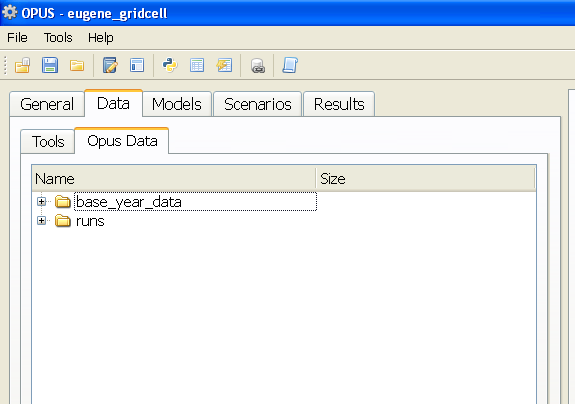
\includegraphics[scale=0.6]{part-gui/images/data-manager-opus-data-tab.png}
\end{center}
\caption{The Opus Data Tab}
\label{fig:opusdatatab}
\end{figure}

There could be any number of subfolders here, but by default you will find
a \file{base_year_data} folder\index{base\_year\_data}, and a \file{runs} folder\index{runs folder}.  The
base_year_data folder will normally contain an Opus \file{database} folder.
An Opus database folder\index{Opus database folder} is any folder containing Opus \file{datasets}.
Often Opus database folders are titled with a year, such as 2000.  Opus
datasets are folders containing Opus `data arrays.'  Opus datasets\index{Opus datasets} are
equivalent to the tables in a database.  Opus data arrays\index{Opus data arrays} are equivalent to
the columns in a table, and are simply numpy arrays that have been written
to disk in a binary format.  See Figure \ref{fig:db-dataset-array}.

\begin{figure}[htp]
\begin{center}
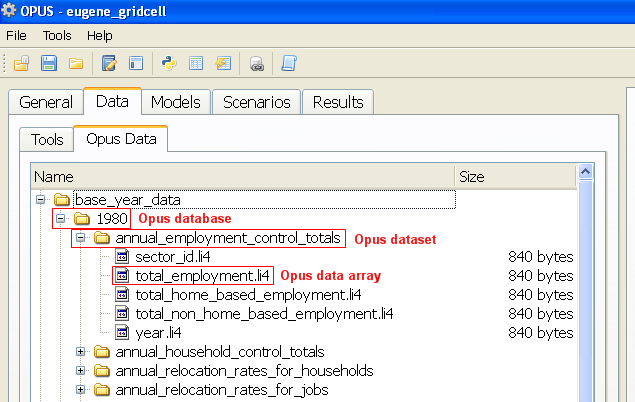
\includegraphics[scale=0.6]{part-gui/images/data-manager-opus-data-tab-db-dataset-array.png}
\end{center}
\caption{Opus databases, datasets, and arrays}
\label{fig:db-dataset-array}
\end{figure}

The Opus data arrays are referred to throughout the documentation as
`primary attributes.'  Primary attributes are the actual data columns in a
dataset.  Computed attributes are attributes computed from primary
attributes via expressions.  For instance, if a parcels dataset contained
the primary attributes population and area, a computed attribute called
population_density could be computed by using the expression
\variable{population_density = population/area}.  Once this expression is
entered and stored in your project in the Variable Library, it can be used
in a model and would be computed as needed.  See Chapter~\ref{chapter:expressions} 
for more details on expressions.

\subsection{Viewing and Browsing an Opus Data table}
To view and browse the contents of an Opus dataset\index{viewing datasets}, right-click a data table, then select 'View Dataset'.  This will bring up a new tab on the right-hand side of the Opus GUI window that will display some summary statistics about the dataset, and a table view of the raw data that can be browsed and sorted by clicking the column name.  See Figure \ref{view-and-browse} for an example of browsing a data table.

\begin{figure}[htp]
\begin{center}
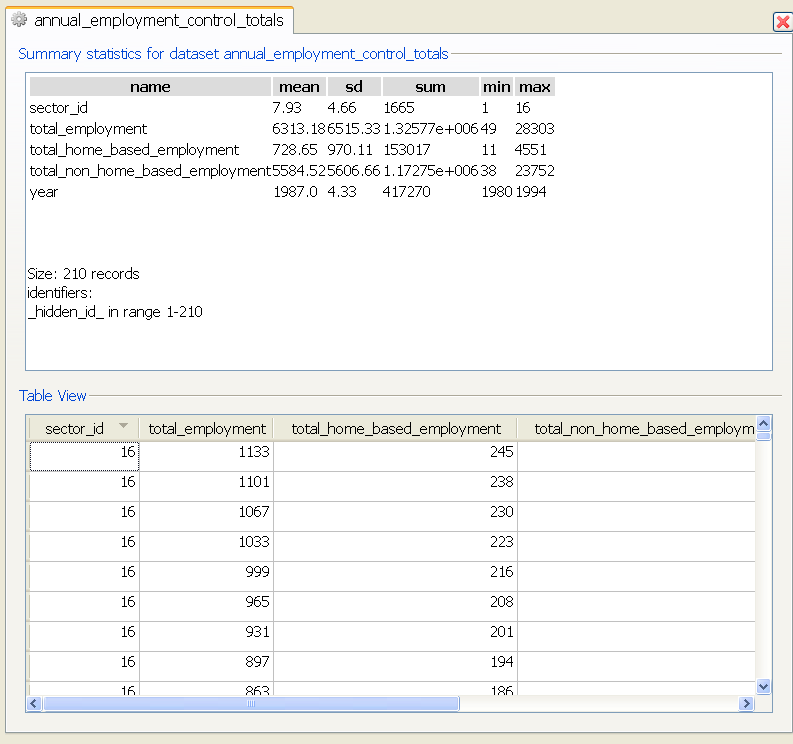
\includegraphics[scale=0.5]{part-gui/images/data-manager-opus-data-tab-view-dataset-tab.png}
\end{center}
\caption{Viewing and browsing an Opus dataset}
\label{view-and-browse}
\end{figure}

\subsection{Exporting an Opus Data table}
An Opus dataset can be exported\index{exporting Opus dataset} to another format for use in other applications.  By default there are 3 options: ESRI, SQL, and CSV.  To export a dataset, right-click a dataset, choose 'Export Opus dataset to,' then click your choice.  See Figure \ref{exporting} for the right-click menu.  You will then see a pop-up window with the respective export tool with the parameters partially filled in based on which dataset you clicked.  These are the same tools that you will find in the Tools tab of the Data Manager.  For more information on the individual tools see the help tab on each tool.

\begin{figure}[htp]
\begin{center}
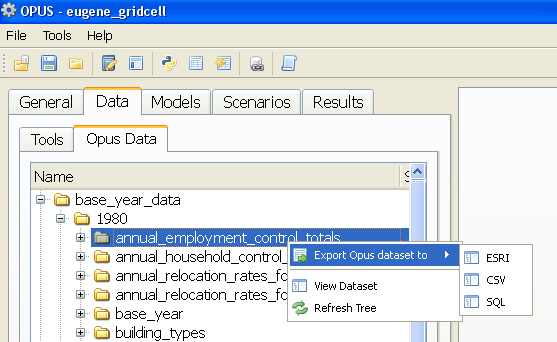
\includegraphics[scale=0.8]{part-gui/images/data-manager-opus-data-tab-export-dataset.png}
\end{center}
\caption{Exporting an Opus dataset}
\label{exporting}
\end{figure}

\section{Tools Tab}\index{Tools tab}\index{Graphical User Interface (GUI)!Tools tab}

The Tools tab\index{Tools tab} is an area to collect and execute tools and batches 
of tools provided with the interface, or it can be extended with tools that you  write.  
A Tool is simply any script that is written in Python and executed by the interface.

\subsection{Tool Library}
The Tool Library\index{Tool library} is a place to collect and organize your tools.  Tools can also be executed directly from the library in a 'one-off' manner, meaning that you can supply parameters to the tool and execute it without storing those parameters for future use.  To execute a tool from the library, simply right-click it and choose 'Execute Tool...', see Figure \ref{execute-tool}.  This will pop-up a window in which you can supply parameters to the tool then execute it.

\begin{figure}[htp]
\begin{center}
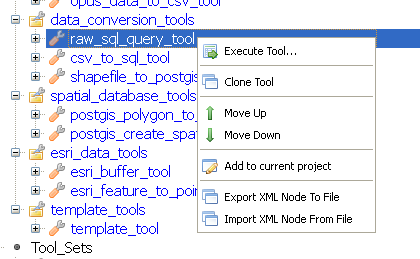
\includegraphics[scale=0.8]{part-gui/images/data-manager-opus-tools-tab-execute-tool.png}
\end{center}
\caption{Executing a tool}
\label{execute-tool}
\end{figure}

\subsubsection{Extending the Tool Library}
New tools can be written and added to the tool library fairly easily.  The best way to explain this is to use an example.  A 'template_tool' has been provided so you can see how it works.  Feel free to execute the template_tool, it just implements a simple loop and prints the results to the tool's log window.  The template_tool's code and associated XML display everything that is needed to add a tool to the interface.  See the code in the source code tree at /opus_gui/data_manager/run/tools/template_tool.py.  A tool also needs XML configuration data in an Opus project.  To view the XML configuration data for the template_tool, open urbansim.xml in an XML editor from the source code tree at /urbansim/configs and search for template_tool.

At the time of this writing new tools must be placed in the source tree at /opus_gui/data_manager/run/tools in order to run correctly.  There are plans to create an additional 'user tools' folder where tools could also be placed.  Also, at this moment, the XML must be hand written to ensure that the tools show up properly in the interface and execute correctly.  There are some right-click functions in the Tool Library to assist with the XML editing (to add a new tool, create parameters for it, etc.) but these functions are in a beta state.

Once a new tool and its associated XML is written properly, the Tool Library will display the tool and dynamically populate the pop-up dialog box with the proper parameters based on the XML configuration.  The tools are quite flexible.  Although the initial tool must be written using Python, there is no limit placed upon what one can do.  For starters, there are tools provided in the interface that make OS calls to external executables (e.g. ogr2ogr.exe), databases, and myriad other libraries to accomplish various tasks (e.g. ESRI geoprocessing).  Feel free to browse the source code for any provided tool along with the XML configuration to see some possibilities.

\subsection{Tool Sets}
Tool Sets\index{Tool sets} are simply collections of tools from the Tool Library with parameters stored so they can be executed repeatedly or in order in a batch manner.  Tool Sets can contain any number of tools from the Library.  A new Tool Set can be created by right-clicking Tool_Sets and choosing 'Add new tool set.'\index{adding new tool set}  This adds a new Tool Set to the bottom of the list.  It can be renamed\index{renaming new tool set} by double-clicking it and typing in a name, taking care to not use spaces or a leading integer as these are invalid in XML nodes.  Once you have a new Tool Set, tools from the Library can be added to it by right-clicking a Tool Set and choosing 'Add Tool to Tool set.'  See Figure \ref{addtool} for an example of what this looks like.

\begin{figure}[htp]
\begin{center}
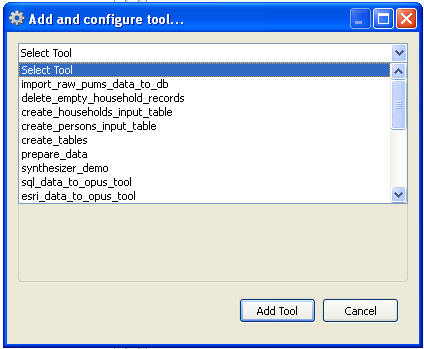
\includegraphics[scale=0.8]{part-gui/images/data-manager-opus-tools-tab-add-tool-to-tool-set.png}
\end{center}
\caption{Adding a tool to a Tool Set}
\label{addtool}
\end{figure}

From this window, choose a tool from the drop down menu, fill in the parameters, then click 'Add Tool.'  The tool is added to the Tool Set and the parameters you entered are stored in the project XML file.  This configured tool can now be executed by itself with those parameters, or executed as part of a batch in the Tool Set.  Tools in a Tool Set can be re-ordered by right-clicking them and choosing to move them up or down, and all of the tools can be executed in the order they appear by right-clicking a Tool Set and choosing 'Execute Tool Set'.
